
\documentclass{ctexart}
\usepackage{amsmath,amsthm,amssymb,amsfonts}
\PassOptionsToPackage{hyphens}{url}\usepackage[colorlinks,linkcolor=blue,anchorcolor=blue,citecolor=blue,]{hyperref}

\usepackage{slashed}
\usepackage{cancel}

\usepackage{graphicx} %插入图片的宏包
\usepackage{float} %设置图片浮动位置的宏包
\usepackage{subfigure} %插入多图时用子图显示的宏包
\usepackage{tikz}
%\usetikzlibrary{positioning, shapes.geometric}
\usetikzlibrary{graphs, positioning, quotes, shapes.geometric}
\usepackage{enumerate}

\usepackage{listings}

\title{QT}
\author{mg21220007}
\date{October 2022}

\begin{document}
\tableofcontents%目录
\maketitle

\section{绪论}
Photon reconstruction and identification seek to  distribution converted and unconverted photons.Unconverted and converted Photons are treated individually in both the reconstruction step,where an attempt is made to classify each correctly,and in the identification step,where different criteria are used for converted and unconverted photons.
\section{AOD,DAOD,xAOD,xDAOD,Ntuples}
AOD (Analysis Object Data), DAOD (Derived Analysis Object Data), xAOD (eXtended Analysis Object Data), xDAOD (eXtended Derived Analysis Object Data), and ntuples are all data formats used in particle physics for storing and analyzing experimental data.

Here are the main differences between these formats:

AOD: This is a data format that contains all the reconstructed objects and events recorded by an experiment. It includes information on particle tracks, energy deposits, and other measurements. AOD is a primary data format that is used for many analyses.

DAOD: This is a format that is derived from AOD. It is produced by selecting specific objects or events from the AOD, and applying additional analysis requirements or algorithms to the selected data. DAOD is often used to reduce the data size, improve signal-to-noise ratios, or add additional information to the data.

xAOD: This is a more compressed and optimized version of AOD. It contains only the most important information needed for analysis, while AOD contains a more complete set of data. xAOD is designed to be more lightweight and easily accessible, allowing for faster analysis and data processing.

xDAOD: This is a derived format that is produced from xAOD. It contains a subset of data that is selected based on specific analysis requirements or algorithms, and is further optimized for faster processing.

BAOD: 
Ntuples: These are data structures that are used to store physics data in a flat format, with each row corresponding to a single event or object. Ntuples are commonly used for analysis and are often produced from AOD or xAOD data formats.


In summary, AOD is the primary data format that contains all reconstructed objects and events, while DAOD, xAOD, and xDAOD are derived formats that are produced by selecting or optimizing specific subsets of data. Ntuples are flat data structures commonly used for analysis.


\section{AOD,DAOD,xAOD,BxAOD,BDxAOD,DxAOD,,ntuple}
\subsection{AOD (Analysis Object Data)}
\begin{enumerate}
    \item AOD is a high-level data format that contains reconstructed physics objects, such as particles, jets, electrons, muons, etc.
    \item AOD files are typically produced after the reconstruction and calibration steps in the data analysis chain.
    \item AOD files are used for a wide range of physics analyses, including event selection, physics object identification, and kinematic studies.
\end{enumerate}

\subsection{DAOD (Derived Analysis Object Data)}
\begin{enumerate}
    \item DAOD is a derived version of AOD, produced by further selecting specific physics objects or applying additional analysis-specific criteria.
    \item DAOD files are smaller in size compared to AOD, as they contain a reduced set of physics objects and variables tailored for specific analysis needs.
    \item DAOD files are optimized for specific physics analyses, allowing for faster data processing and reduced storage requirements.
\end{enumerate}

\subsection{xAOD (eXtensible Analysis Object Data)}
\begin{enumerate}
    \item xAOD is an extension of AOD that provides a more flexible and extensible data format.
    \item xAOD files introduce a standardized data model and interface for accessing physics objects and related information.
    \item xAOD allows for the inclusion of additional analysis-specific variables and objects through an extensible framework.
\end{enumerate}

\subsection{BxAOD (Base eXtension Analysis Object Data)}
\begin{enumerate}
    \item BxAOD is an extended version of xAOD that includes additional branches or variables not present in the standard xAOD.
    \item BxAOD files are typically used for custom analysis needs where specialized variables or branches are required.
\end{enumerate}

\subsection{BDxAOD (Base Derived Analysis Object Data)}
\begin{enumerate}
    \item BDxAOD is a combination of BxAOD and DAOD, which includes both customized variables and a reduced set of physics objects.
    \item BDxAOD files are designed for specific analyses that require a tailored set of physics objects and additional variables.
\end{enumerate}

\subsection{DxAOD (Derived eXtensible Analysis Object Data)}
\begin{enumerate}
    \item DxAOD combines the flexibility of xAOD with the customization of DAOD, providing both an extended data format and analysis-specific selection.
    \item DxAOD files are optimized for specific analyses, with a reduced set of physics objects and customized variables.
\end{enumerate}

\subsection{ntuple}
\begin{enumerate}
    \item An ntuple is a generic term used to refer to a flat, table-like data structure typically stored in ROOT files.
    \item Ntuples contain variables or branches representing various physics quantities, often obtained after event selection and reconstruction.
    \item Ntuples are commonly used in data analysis for easy access and manipulation of data.
\end{enumerate}
\subsubsection{convtype}
\url{https://twiki.cern.ch/twiki/bin/view/AtlasProtected/AtlasPhotonPurity}
\begin{enumerate}
    \item Conversion categories are defined by the detected conversion and the number of reconstructed tracks:\\
    \begin{enumerate}
        \item in AOD, a converted photon has phot->conversion()!=0
        \item from phot->author() one can tell whether the photon was recovered (author==16) or not (author==4)
    \end{enumerate}
    \item in PAU all this is condensed in the two-digit variable ph\_convFlag
    \begin{enumerate}
        \item the left digit (ph\_convFlag\%10) tells the number of tracks (0 means unconverted)
        \item the right digit (ph\_convFlag/10) tells whether the photon was recovered (1) or not (0)
    \end{enumerate}
\end{enumerate}

\subsubsection{truth conversion}
The definition of the truth conversion (for truth photons) is as follows:
\begin{enumerate}
    \item photon must have an end vertex and two children e+, e-
    \item conversion vertex must have radius R<800 mm
    \item both e+.e- must have |eta|<2.5 and pt>500 MeV
\end{enumerate}
\section{about rucio files}
\url{https://rucio.cern.ch/documentation/started/concepts/file_dataset_container#data-identifiers-and-scope}
Files, datasets and containers follow an identical naming scheme which is composed of two strings: the scope and a name. The combination of both is called a data identifier(DID). Thus for files, the Logical File Name(LFN), a term  commonly used in Datagrid terminology to identify files is  equivalent to the DID in Rucio.\\

The scope string partitions the namespace into several sub namespaces. The primary use case for this is to easily separate centrally created data form individual user data.\\

By default, accounts have read access to all scopes and write access only to their own scope. privileged accounts have write access to multiple scopes. e.g.. the Workload Management System is allowed to write into official data scopes.\\

Files, datasets and containers are uniquely identified over all time. This means that a data identifier, once used, can never be reused to refer to anything else at all, not even if the data it referred to has been deleted from the system.

\begin{figure}[H] %H为当前位置,!htb为忽略美学标准,htbp为浮动图形
\centering %图片居中
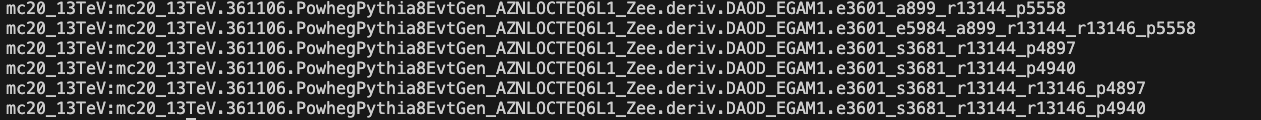
\includegraphics[width=1.0\textwidth]{rucio-file.png} %插入图片,[]中设置图片大小,{}中是图片文件名
\caption{rucio-file} %最终文档中希望显示的图片标题
\label{rucio-file} %用于文内引用的标签
\end{figure}
\subsection{how to use rucio}

\begin{lstlisting}
    rucio list-dids "mc20_13TeV.8006*.*DAOD_*r13145*p5536" |grep CONTAINER
\end{lstlisting}
\subsection{how to upload a file }
rucio upload --scope user.zgao --rse CERN-PROD\_SCRATCHDISK test\_1.root  \\
rucio attach user.zgao:tag\_and\_probe\_prw user.zgao:test\_1.root \\
rucio list-files user.zgao:tag\_and\_probe\_prw\\
rucio list-file-replicas user.zgao:test\_1.root
\subsection{what's the meaning of its name(AMI tags)}
\url{https://twiki.cern.ch/twiki/bin/view/AtlasProtected/AtlasProductionGroupMC20}\\
\url{https://twiki.cern.ch/twiki/bin/view/AtlasProtected/AtlasProductionGroup}\\
\url{https://twiki.cern.ch/twiki/bin/view/AtlasProtected/AtlasProductionGroupMC16eExtra}
\begin{enumerate}[1)]
\item EVNT-merge tags
\item s-tag for simulation
\item s-tag for sim-merge
\item d-tag for digi
\item r-tag for digi+reco
\item r-tag for rec-merge
\item a-tag for Atlfast
\item a-tag for Atlfast's digit=reco
\item p-tags
\end{enumerate}
\subsubsection{simulation}
s stands for full simulation\par
a stands for fast simulation
\subsubsection{reconstruction}
r13167 recon (overlay+trigger+reconstruction) for MC20a\par
r13144 recon (overlay+trigger+reconstruction) for MC20d\par
r13145 recon (overlay+trigger+reconstruction) for MC20e
\subsubsection{pile-up presampling}
d1713 MC20a RDO production \par
(mc20\_ 13TeV.900149.PG\_ single\_ nu\_ Pt50.digit.RDO.e8307\_ s3482\_ s3136\_ d1713)\par
d1714 MC20d RDO production \par
(mc20\_ 13TeV.900149.PG\_ single\_ nu\_ Pt50.digit.RDO.e8307\_ s3482\_ s3136\_ d1714)\par
d1715 MC20e RDO production \par
(mc20\_ 13TeV.900149.PG\_ single\_ nu\_ Pt50.digit.RDO.e8307\_ s3482\_ s3136\_ d1715)

\subsubsection{special tags }
r13146 AOD merge\par
p4836 NTUP\_ PILEUP creation\par
p4837 NTUP\_ PILEUP merge\\

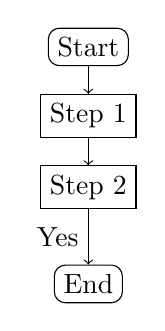
\begin{tikzpicture}[node distance=10pt]
  \node[draw, rounded corners]                        (start)   {Start};
  \node[draw, below=of start]                         (step 1)  {Step 1};
  \node[draw, below=of step 1]                        (step 2)  {Step 2};
  %\node[draw, diamond, aspect=2, below=of step 2]     (choice)  {Choice};
  %\node[draw, right=30pt of choice]                   (step x)  {Step X};
  \node[draw, rounded corners, below=20pt of step 2]  (end)     {End};
  
  \graph{
    (start) -> (step 1) -> (step 2) ->["Yes"left] (end);
    %(start) -> (step 1) -> (step 2) -> (choice) ->["Yes"left] (end);
    %(choice) ->["No"] (step x) ->[to path={|- (\tikztotarget)}] (step 2);
  };
\end{tikzpicture}
\paragraph{p tag}

\section{DxAOD Derivation}
\subsubsection{AMI URL}

\subsection{EGAM1~10}
\url{https://ami.in2p3.fr/?subapp=document}
\begin{enumerate}
    \item EGAM1  Z->ee reduction for central electrons - for electron ID and calibration
    \item EGAM2  J/psi->ee derivation for calibration
    \item EGAM3  Z->eegamma reduction for low-pT electron and photon studies
    \item EGAM4  Z->mumugamma and mumue reduction for photon (and fake photon->e) studies
    \item EGAM5  W->enu derivation
    \item EGAM6  
    \item EGAM7  electron selection, to retain fake electron candidates,Cell collection is saved but thinned (keep only cells associated with egammaClusters)
    \item EGAM8  Z->ee reduction for forward e tag-and-probe (one central e, one fwd e), Z->emu reduction for bkg studies (one mu, one fwd e)
    \item EGAM9  keep events passing or of photon triggers used for boostrap efficiency, measurement of photon triggers
    \item EGAM10 Inclusive photon reduction - for e/gamma photon studies
    \item EGAM11 Z->ee reduction for central electrons - for electron ID and calibration, Adaptation of EGAM1 for heavy ions
    \item EGAM12 Keep events passing OR of electron triggers, or inclusive electron selection, to retain fake electron candidates. Adaptation of EGAM7 format for heavy ion runs (no triggers, no pflow jets, extra containers)


\end{enumerate}
\subsection{STDM2}
\subsection{JETM}
This package contains the derivation formats (JETMX) needed for Jet/Etmiss performance studies.
\begin{enumerate}
    \item JETM1.py:  MC calibrations (MC-JES, GSC) and in situ calibrations (eta-intercalibration, MJB, JER), trigger jet studies
    \item JETM2.py: MC only for tagger developments, JetDef R\&D (rho, towers, ...), this is a merged format of JETM8 and JETM13
    \item JETM3.py: in situ Z+jets calibration
    \item JETM4.py: in situ gamma+jets
    \item JETM5.py: random cones in zero bias data
    \item JETM6.py: tagging scale factors
    \item JETM10.py: MET trigger studies
    \item JETM11.py: MET trigger studies in e+mu events
    \item JETM12.py : E/p studies in W to tau + nu events
    \item JETM14.py: MET trigger studies in single lepton events
\end{enumerate}
\subsection{FTAG}
\section{ATLAS package dependency viewer }
\url{https://atlas-sw-adeps.web.cern.ch/atlas-sw-adeps/}
\section{why we need photon ID}
Studying of the rare physics processes with photons in the final state occurring in proton-proton collisions play a central role of the LHC physics programme. These include the diphoton decays of recently discovered Higgs bosons with a mass around 125GeV,as well as the process expected from BSM scenarios,such as the resonant photon pairs from gravition decays,photon pairs in association with large missing energy from the decays of pairs of supersymmetric particles,etc. The study of non-resonant production of single photons(produced mainly via quark-gluon Compton scattering and quark-antiquark annihilation) in association with jests allows to test pertubative (fixed-order calculations) and non-perturbative (ressummed calculations,parton shower approaches)domains of QCD and can provide useful information about the PDFs. It is essential to have accurate predictions of such process as they represent an important background to Higgs boson production and the BSM searches.

\section{Photon ID is challenging}
The identification of prompt photons in hadronic collision is particularly challenging, since the overwhelming  majority of reconstructed photon candidates arise from background non-prompt photons from hadron decays in jets, while a smaller fraction of fake candidates are associated with hadrons that deposit significant energy in the electromagnetic calorimeter, mimicking that of real photons

\section{why should we classify converted and unconverted}
The shower differs for photons that do(converted) or don not(unconverted) to electron-positron pairs in the detector material upstream of EM calorimeter.  \par
to account for the calorimeter geometry and  for different effects on the shower shapes from the materal upstream of the calorimeter,the studies are  performed ins seven pseudorapidity regions $|\eta|$ of the dector.\par
The optimization of tight ID menu is done separately for converted and unconverted photons,as their showers differ due to opening azimuth angle between the conversion electrons appearing in the solenoid field.

\section{how to identify}
Prompt photons are identified in the ATLAS experiment by means of selections on quantities describing the shape and properties of the associated electromagnetic showers, and by requiring them to be isolated from other particles in the event.The selections are separately optimised for those photon candidates that converted and unconverted.
\section{terminology}
\subsection{(scale factor)SF}
eff(data)/eff(MC)
\subsection{cut} selection criteria
\subsection{prescale trigger}
\subsection{template fit}
\subsection{硬散射过程}

\subsection{部分子簇射}
部分子簇射是部分子在硬散射结束后的传播过程中因为真空涨落效应引起的一系列辐射过程。该过程可以被分为因色荷(强相互作用)引起的强子辐射过程和因电荷(电磁相互作用)引起的电磁辐射过程。其中电磁辐射过程一般被归纳为初态辐射过程。
\subsection{强子化过程}
当部分子的能量不足以产生新的簇射之后,部分子因"色禁闭"效应需要彼此之间U成"无色"的粒子态(强子),这一过程被称为强子化过程。
\subsection{潜在事例underlying event}
\subsection{pile-up effect}
\subsubsection{in-time pile-up}
在同一个粒子簇团中发生的多个质子-质子硬散射碰撞。
\subsubsection{out-of-time pile-up}
在不同粒子簇团中发生的多个质子-质子硬散射碰撞。
一般用<$\mu$>来表示每个簇团截面中的质子-质子硬散射碰撞的平均事例数.\par
事例的堆积效应可以通过堆叠多个模拟产生pp对撞样本来模拟。然后给堆叠的样本一个额外的权重去符合实际过程中的堆积效应。这一过程一般被称为"pile-up reweighting".
\subsubsection{pileupreweight,PRW}
average mu $<mu>$ is averaging the ' actual mu; over the colliding bunches \par
'actual mu' (or just mu ) is the mean number of minbias collisions.\par
but in MC , $<mu>$ = mu (all neighbouring bunches in a simulated event are given the same mu as the central event)\par
in data, $<mu>$ is NOT equal to mu 
\subsection{Topological clusters(拓扑簇)(Chat Gpt)}
"Topological clusters"(拓扑簇)是指在粒子物理实验中用于重建粒子轨迹的一种数据处理技术。在高能物理学和粒子物理学实验中,探测器通常会记录粒子与探测器相互作用产生的能量沉积(能量簇)信息。而 "topological clusters" 就是基于拓扑学原理,将这些能量沉积信息组合成更大、更完整的粒子轨迹的一种方法。

"Topological clusters" 可以理解为一组相邻且相互连接的能量沉积,通常在探测器中形成一个连通的区域,被认为可能是同一粒子轨迹上的能量沉积点。这种方法基于探测器中相邻的能量沉积点在物理上可能对应于粒子轨迹上的相邻点的原理,通过将这些能量沉积点连接在一起,可以重建粒子的轨迹信息,从而对粒子进行鉴别和测量。

"Topological clusters" 在粒子物理实验中用于粒子轨迹重建和事件重建的过程中起着重要作用,对于研究粒子的性质、相互作用和动力学等方面具有重要的应用价值。具体的实现方式和算法可能因实验和探测器的不同而有所不同,因此在具体的实验和文献中,"topological clusters" 的具体含义和用法应根据上下文和实验情境来解释。
\subsection{isolation}
在粒子物理中,隔离(isolation)是一种重要的重建算法,用于区分单个粒子与其周围的其他粒子或背景事件。隔离通常是通过测量在以该粒子为中心的一个小区域内的粒子能量来实现的。\\

The definition of photon isolation in ATLAS is based on the transverse energy in a cone with angular size $\Delta R$ around the direction of the photon candidate. This transverse energy is characterized by two quantities, the calorimeter isolation and the track isolation.
\subsubsection{calorimeter isolation $E_T^{iso}$,$topocone$}
topocone 是一种重建算法,用于在以某个对象为中心的圆锥形区域内,使用拓扑刻度来计算所有粒子的横向动量之和。与 ptcone 和 etcone 不同,topocone 不仅考虑了在圆锥形区域内具有高动量或高能量的粒子,还考虑了较低能量的粒子和多个粒子的相互作用。因此,topocone 通常用于在复杂的物理环境中,对于具有高动量或高能量的粒子的鉴别和分类。\\

etcone 是一种重建算法,用于计算在以某个对象为中心的圆锥形区域内,所有具有足够高的能量的粒子(例如光子或中性粒子)的横向能量之和。因此,etcone 值通常用于对于具有高横向能量的粒子(例如光子或衰变轻子)的鉴别和分类。\\


The calorimeter isolaiton $E_T^{iso}$ is obtained from the sum of transverse energies of topological clusters in the calorimeters , after subtracting on an event-by-event basis the energy deposited by the photon candidate and the contribution from the underlying event and pile-up.

1.首先,我们选择一个半径为 $R$ 的圆锥形区域,以待测粒子的位置为中心。\par
2.接着,我们计算该圆锥形区域内所有的能量总和,包括来自待测粒子和其他粒子的能量。这里的能量可以是电磁能量、强子能量或总能量等不同类型的能量。\par
3.最后,我们将这个总能量与一个预先定义的阈值进行比较。如果总能量小于阈值,我们就可以认为该待测粒子是孤立的,否则就认为它被其他粒子或背景事件所隔离。\par

\paragraph{etcone和topocone的区别}
在粒子物理实验中,topocone 是一种算法,用于测量和鉴别不同种类的高能粒子。和 etcone 算法一样,topocone 算法也是一种圆锥形的隔离算法,其基本思想是在以待测粒子为中心的圆锥形区域内,测量粒子沉积的能量总和,并与预先定义的阈值进行比较。

相对于 etcone 算法,topocone 算法有更高的空间分辨率和更好的能量重建性能,特别是在探测器前端的粒子沉积区域(EM cluster)中,能够更准确地鉴别电子和光子。因此,在需要进行高精度测量或区分不同种类的粒子时,通常使用 topocone 算法来替代 etcone 算法。同时,topocone 算法也更适用于高能物理实验,由于高能粒子和背景事件之间的区别更加微妙和复杂,需要更准确和可靠的测量手段来区分它们。
\subsubsection{track isolaiton $p_T^{iso}$}
在粒子物理中,Track isolation 是一种隔离(isolation)算法,用于区分单个带电粒子与其周围的其他粒子或背景事件。Track isolation 通常是通过测量在以该带电粒子为中心的一个小区域内的轨迹的总长度来实现的。\\

ptcone 是一种重建算法,用于计算在以某个对象为中心的圆锥形区域内,所有具有足够高的动量的粒子(例如带电粒子)的横向动量之和。因此,ptcone 值通常用于对于具有高横向动量的粒子(例如喷注)的鉴别和分类。\\

1.首先,我们选择一个半径为 $R$ 的圆锥形区域,以带电粒子的位置为中心。\par
2.接着,我们计算该圆锥形区域内所有的轨迹长度之和,包括来自带电粒子和其他粒子的轨迹。这里的轨迹长度可以用以下公式计算:
$$\sum_{tracks_i}p_{T,i}\times\Delta R_{i,j}$$
其中 $p_{\text{T},i}$ 是第 $i$ 条轨迹的横向动量,$\Delta R_{i,j}$ 是第 $i$ 条轨迹与带电粒子之间的 $\Delta R$ 距离,即:
$$\Delta R_{i,j}=\sqrt{(\eta_i-\eta_j)^2+(\phi_i-\phi_j)^2}$$
其中 $\eta$ 和 $\phi$ 分别是轨迹的赝快度和方位角.\par
3.最后,我们将这个总长度与一个预先定义的阈值进行比较。如果总长度小于阈值,我们就可以认为该带电粒子是孤立的,否则就认为它被其他粒子或背景事件所隔离。

The track isolation $p_T^{iso}$ is obtained by summing the transverse momenta of all the tracks with transverse momentum above 1 GeV and having a distance of closet approach to the primary vertex along the beam axis $\left|z_0 sin\theta \right| < 3$ mm, and excluding the track associated with photon conversions.\\


\medskip
\begin{figure}[H] %H为当前位置,!htb为忽略美学标准,htbp为浮动图形
\centering %图片居中
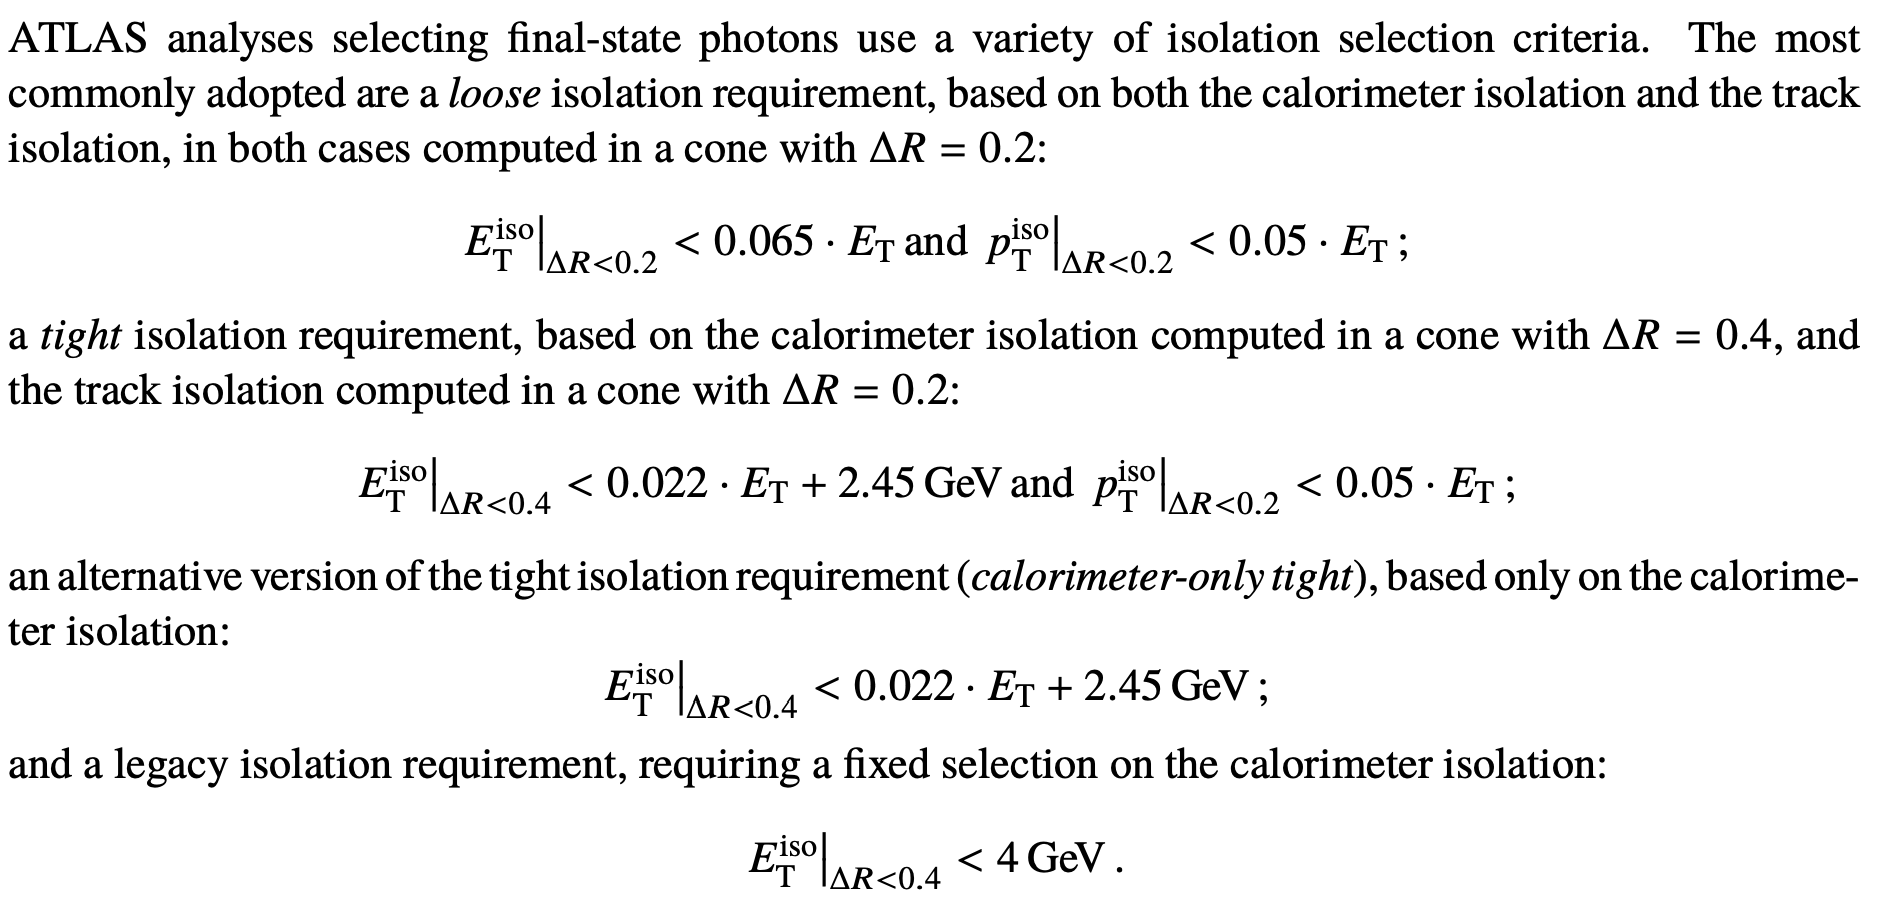
\includegraphics[width=1.0\textwidth]{isolation.png} %插入图片,[]中设置图片大小,{}中是图片文件名
\caption{Isolation} %最终文档中希望显示的图片标题
\label{Isolation} %用于文内引用的标签
\end{figure}

\subsection{luminosity (instantaneous luminosity)}
luminosity, which gives the number of particles in each beam that crosses a unit area in unit time. Sometimes it is called instantaneous luminosity in order to distinguish it from integrated luminosity
\section{system uncertainty}
\subsection{closure test}


$\mathbf{RADZ}$:A closure test is made by performing the measurement on
a sample consisting of known fractions of simulated signal
and background events. This test is only performed for
ET < 25 GeV, because of the the limited number of MC
events at higher transverse momenta. Deviations from the
true identification efficiency are included as systematic
uncertainties. Their value is below 1\% in all regions.
\par$\mathbf{EE}$:A closure test of the Smirnov transform procedure is
performed by comparing photon identification efficiencies
for transformed MC electrons and MC photons. This
check accounts in particular for a difference in the correlations
of shower-shape variables between photons and
electrons, which are not modified by the per-variable
Smirnov transforms. The effect is found to be at most
1\% for converted photons and 2\% for unconverted photons.
\par$\mathbf{MM}$:A closure check on the computation of the background
efficiencies 
total
bkg and 

pass
bkg is performed by determining
their values as described above in a sample of simulated
multijet production (see Sect. 4). The relative differences
between these values and the true value is used as a systematic
uncertainty. The uncertainty reaches 18\% at low
ET but is about 3\% at 50 GeV and below 1\% at high ET.
\subsubsection{what's the meaning of closure test}
CERN Atlas(欧洲核子研究中心的一个实验项目)中的"closure test"是指一种用于评估实验数据处理和分析的方法。在高能物理实验中,科学家们使用复杂的数据处理和分析技术来研究粒子的相互作用和性质。

"closure test"是一种验证数据处理和分析方法是否有效的测试方法。它通常通过在已知的模拟数据上进行测试,然后与预期结果进行比较来完成。这种测试可以帮助科学家们确认他们的数据处理和分析程序是否正确地处理了实验数据,是否能够从复杂的原始数据中正确地提取出物理信息。

在CERN Atlas实验中,"closure test"可能涉及使用已知的模拟数据作为输入,通过实验的数据处理和分析链,生成预期的输出结果。然后,这些输出结果可以与预期结果进行比较,以验证数据处理和分析方法是否在预期范围内工作,从而确定实验的准确性和可靠性。这有助于科学家们确认他们的实验数据是否能够产生可靠的物理结果,从而支持他们的科学研究和结论。
\paragraph{来自陈汇润师兄的看法}
一般地说就是做测量有一个control 样本,你用这个控制样本测量一个scale factor或者诸如此类的东西,再把这个SF应用回去这控制样本上,看data和你SF修正过的mc 是不是吻合,这中就叫closure test。
\subsection{background}
$\mathbf{RADZ}$:An uncertainty in the level of background contamination
is assessed by computing εID with and without accounting
for the background component, and using the differences
between the two results in each region as a systematic
uncertainty. Its values are less than 2.5\%, except in
the region $E_T$ < 15 GeV where they are as large as 8\%.
\par$\mathbf{EE}$:An uncertainty is assigned to the background subtraction
technique by repeating the measurement while using the
range 80 < $m_ee$ < 100 GeV for the template fit. The
difference between this result and the nominal result is
used as a systematic uncertainty.
\par$\mathbf{MM}$:
\subsection{generator}
$\mathbf{RADZ}$:Similarly to the above, the generator used in the signal
simulation is changed from Sherpa to POWHEG-BOX.
The impact of this change on the computed εID is typically
3\% or less except for ET < 15 GeV where it is as
large as 10\%, and is included as a systematic uncertainty.
\par$\mathbf{EE}$:
\par$\mathbf{MM}$:
\subsection{isolation}
$\mathbf{RADZ}$:
\par$\mathbf{EE}$:
\par$\mathbf{MM}$:An uncertainty due to the tight isolation requirement is
evaluated by changing the size of the isolation cone from
0.4 to 0.2. The uncertainty reaches 8\% at low ET, but is
less than 1\% above 50 GeV.
\subsection{conversion}
$\mathbf{RADZ}$:
\par$\mathbf{EE}$:
\par$\mathbf{MM}$:
\subsection{fragmentation}
$\mathbf{RADZ}$:
\par$\mathbf{EE}$:
\par$\mathbf{MM}$:
\subsection{Fudge factor}
1. Fudge factors are used to correct the shower shape variables in MC in order to fit the observed distributions in data.\par
As the correction factor is estimated from prompt photon MC.possible difference of the loose ID and trigger efficiencies in data and MC are not accounted for.\par
2. Data-to-simulation efficiency ratio used as correction factors in physicals measurements are determined to accounted for the small residual efficiency differences.\par
3.The shower shape distributions in simulation are shifted by so called  fudge factors to match the distribution founded in data.\\
Fudge factors are used to correct the shower shape variables in MC in order to fit the observed distributions in data.


$\mathbf{RADZ}$:
\par$\mathbf{EE}$:
\par$\mathbf{MM}$:
\subsection{StatMC}
$\mathbf{RADZ}$:
\par$\mathbf{EE}$:
\par$\mathbf{MM}$:
\subsection{Correction factor}
Two individual uncertainties are combined for the uncertainty that are related to the correction factor.\par
The trigger correction factor ,obtained from the ratio of the isolated photon tight identification efficiencies without and with trigger requirement in simulated prompt photon samples(after applying fudge factors to the shower shape variables). \par
Since the photon triggers apply some(loose) requirements on the electromagnetic shower shapes,they may bias the ID efficiency measurement,especially at low transverse momentum.A correction factor is therefore applied in the end in order to take this effect into account. \par
In this study, since the inclusive photon triggers are used for the preselection of the sample, what
is measured with the preselected sample is the tight identification efficiency for photon candidates passing
the shower shape requirements applied by the trigger
$$\epsilon '=\frac{N_\gamma^{tight,reco,trig}}{N_\gamma^{reco,trig}}$$
while we are interested in the tight identification efficiency for all reconstructed photons:
$$\epsilon=\frac{N_\gamma^{tigger,reco}}{N_\gamma^{reco}}$$
We can obtain the latter from the former by applying a multiplicative factor
$$\epsilon=\epsilon'\frac{\frac{N_\gamma^{tight,reco}}{N_\gamma^{reco}}}{\frac{N_\gamma^{tight,reco,trig}}{N_\gamma^{reco,trig}}}=\epsilon'\frac{\frac{N_\gamma^{trig,reco}}{N_\gamma^{reco}}}{\frac{N_\gamma^{tight,reco,trig}}{N_\gamma^{reco,trig}}}$$
The correction factor,is the ratio between the tight ID efficiency for all reconstructed photons or only for photons matching the trigger object that triggers the event, as obtained  from simulated direct photon samples after correcting the shower shapes by the fudge factors.
$\mathbf{RADZ}$:
\par$\mathbf{EE}$:
\par$\mathbf{MM}$:
\subsection{others from RADZ}
An uncertainty in the description of the detector in simulation
is assessed by using an alternative geometry with
additional inactive material in front of the calorimeter
when obtaining the simulated signal distribution. The
amount of additional material is chosen to be compatible with the measurements performed using Run 1 data [19].
The determination of εID is repeated with this configuration,
and the relative changes in the results for each
region are counted as systematic uncertainties. Their values
are typically below 2\%, but up to 5\% in the endcap
and negligible for ET > 25 GeV. 
\subsection{others from MM}
\subsubsection{1}
An uncertainty due to the description of the detector in
simulated samples is derived in the same way as for the
method using radiative Z decays, using samples with
variations in the amount of inactive material in front of
the calorimeter. The size of the uncertainty is typically
1\% at low ET and at the per-mil level at high ET, except
for the unconverted photons in the first endcap bin where
uncertainties reach 4%.
\subsubsection{2}
The statistical uncertainties in the simulation samples are
accounted for using the electron extrapolationmethod by
iteratively resampling the corresponding datasets, and are
typically 0.5\% or less.
\subsection{other from EE}
\subsubsection{1}
An uncertainty is assigned because of the difference in
the fraction of converted photons between data and simulation,
which impacts the simulated shower shapes used
to derive the Smirnov transforms. The fraction of true
converted photons in the simulated photon sample is
varied by ±10\%, an amplitude which covers the differences
between data and simulation reported in Sect. 7;
the resulting change in εID is used to estimate the uncertainty.
The effect is of the order of 0.2\% or less, and up
to about 1\% in the first endcap $|\eta|$bin.
\subsubsection{2}
As described in Sect. 4.1, shifts are applied to simulated
shower shape distributions to align them with those in
data. These do not, however, capture the full difference
between data and simulation if the shapes cannot be reconciled
by simple shifts. The impact of the residual differences
is accounted for by defining for each variable a
range of shift values such that, for any value of the variable,
the data distribution can be locally matched to the simulated distribution by a shift belonging to the range of
allowed shift values. The measurement is then repeated
with the endpoints of the range replacing the nominal
value of the shift for each variable. The sum in quadrature
of the maximum changes relative to the nominal
measurement for each variable is used as an uncertainty.
The uncertainties are typically below1\%at low ET.However,
the relatively tight cut on the fside variable in the
1.81 ≤ |η| < 2.37 bin leads to uncertainties of about 5\%
for unconverted photons and 2\% for converted photons.
\subsubsection{3}
An uncertainty is assigned to the fraction of photons originating
from fragmentation processes in the simulation.
These photons are less isolated than direct photons and
have broader showers, which affects the Smirnov transforms.
The uncertainty is computed as the variation in εID
when the number of fragmentation photons is varied by
± 50\% in simulation. The uncertainty is typically 0.3\%
or less, rising to 1\% at high ET.
\subsubsection{4}
Finally, an uncertainty is assigned to account for statistical
uncertainties in the simulation sample. The uncertainty
is computed by iteratively resampling the simulated
samples, recomputing εID for each iteration, and the uncertainty is extracted as the width of the resulting
distribution. The uncertainties are typically 0.3\%, and up
to 0.6\% at high ET.
\subsection{conclusion}
$\mathbf{RADZ}$:The statistical uncertainty is obtained from the $m_{ll\gamma}$ shape
fit. It remains typically below 1\% for ET < 40 GeV but rises
to about 5\% at 80 GeV. The total uncertainty reaches 5–15\%
for ET < 15 GeV, about 5\% for 15 < ET < 25 GeV, 1\%
for 25 < ET < 40 GeV and then follows a rise driven by the
statistical uncertainty.
$\mathbf{EE}$:The statistical uncertainty is computed by iteratively resampling
the data as described above for the simulated samples.
It remains below 0.1\% over the range 25 < ET < 150 GeV
covered by this measurement. Overall, the total uncertainty
reaches about 2\% at low ET, and is typically below 1\% for
ET > 40 GeV. However, values of up to 5\% are reached for
unconverted photons in the bin 1.81 ≤ $|\eta|$< 2.37 due to
the data–MC differences noted above in the $f_side$ variable.
$\mathbf{MM}$:The statistical uncertainty is computed as the width of the
distribution of results obtained when repeating the measurement
on pseudo-datasets obtained by resampling the data
and reach 1–2\% for ET < 50 GeV and typically 0.5%
at higher ET. The total uncertainty reaches to 7–18% at
ET = 25 GeV, but 2–3\% at 40 GeV and 1\% or less above
100 GeV except for unconverted photons for ET > 250 GeV
and 1.52 ≤ |η| < 1.81 where it reaches 4\% as noted above.
\section{detector}
ATLAS 的⼦系统从内向外依次为内探测器
(ID,处在2T的轴向磁场中),螺线管电磁铁,电磁量能器(ECal)强⼦量能
器(HCal),繆⼦探测器和三块环形电磁铁
\subsection{inner detector}
处于2T的轴向磁场中
\subsubsection{Pixel,硅像素探测器}
共有4层,最靠近束流管的一层被称为B-Layer,外面的三层被称为Layer-0,Layer-1和Layer-2
\subsubsection{半导体径迹探测器(硅微条探测器,SCT)}
\subsubsection{跃迁辐射探测器(气体探测器,TRT)}
\subsection{螺线管电磁铁}
\subsection{Electromagnetic calorimeter}
简称ECal\\
电磁量能器比强子量能其更加精细,用来精确地测量电子和光子的沉积能量\\
电磁量能器的桶部部分由三层组成。
\subsubsection{第一部分}
第⼀层的深度(r⽅向)约为4 个辐射f
长度($X_0$),它在$\eta-\phi$方向⼗分精细,为$\Delta\eta\phi$ = 0.003x0.1,通过对这⼀层
沉积能量的精确测量可以为电⼦和光⼦鉴别提供信息
\subsubsection{第二部分}
第⼆层的深度为16 个辐
射长度,这⼀层吸收了⼤部分的光⼦-电⼦簇射产物及其能量,这⼀层的粒度为$\Delta\eta\phi=0.025x0.025$
\subsubsection{第三部分}
最后⼀层的深度为2 个辐射长度,尺⼨为$\Delta\eta\phi=0.05x0.025$
这⼀层被设计为吸收残余的光⼦-电⼦簇射。
\subsection{Hadron Calorimeter}
简称HCal
\subsection{Muon Chambers}
\section{photon}
\subsection{inclusive photon}
inclusive photon includes converted photon and unconverted photon

\subsubsection{converted photon}
convert to electron-positron pairs after interacting with detector material in the inner detector.\par
另一种说法: convert into an electron-positron pair before reaching the electromagnetic calorimeter.
Converted(undergoes $e^+e^-$ pair production before ECAL)\par
Converted photons are further categorized into single and double-track conversions,depending on the number of reconstructed tracks.\par
在Atlas实验中,大约20\%的在低$|\eta|$区间的光子都是conversion photon。

A true converted photon is defined as a photon undergoing a conversion into an electron-positron pair within a distance $r < 80  $ cm from the interaction point. 

\subsubsection{unconverted photon}
the photon reaches the calorimeter with  no such interaction.\par
Unconverted(undergoes pair production in ECAL)\par
在$|\eta|$ $\approx2.3$的区间内。超过65\%的光子是通过转换而来
\subsubsection{\textbf{\large what's the meaning of inclusive}}
it means the photon is measured regardless of what else is  produced in the collision
\subsection{prompt photon and background photon}
\subsubsection{prompt photon}
photons not originating from hadron decays. The main contributions come from nonresonant
production of photons in association with jets or
of photon pairs, with cross sections respectively of the order
of tens of nanobarns or picobarns .\par
%\vspace{1cm}
\medskip
Process with prompt photons in the final state. They encompass all phenomena where photons do not originate from hadron decays. These range from non-resonant QCD production, where prompt photons are produced in association with jets or in pairs with cross sections of the order of tens of nanobarns or picobarns respectively, to rarer process where prompt photons arise from the decay of a heavy particle.  
Prompt photons are also produced in rarer processes that are key
to the LHC physics programme, such as diphoton decays
of the Higgs boson discovered with a mass near 125 GeV,
produced with a cross section times branching ratio of about
20 fb at √s = 8TeV.\par
\medskip
Prompt Photons,i.e.  photons not originating from hadron decays, include both direct photons, which originate directly from the hard process, and fragmentation photons, which originate form the fragmentation of high-$P_T$ partons. Fragmentation photons, as a result of the differing production kinematics, tend to be less isolated than direct photons , and their shower shape distributions are usually broader than those of direct photons , as well as of (prompt) electrons.\par
\medskip
There are several different ways photons can be produced in a collision at the LHC. One of the most common is in the decay of neutral pions, which are hadrons created copiously when protons are samshed up.
\paragraph{what's the meaning of prompt}
By "prompt" though , we means photons which are produced promptly in the collision , before the quark and gluons have had time to form hadrons, and well before those hadrons decay.
\subsubsection{non-prompt photon }
如$\pi_0\rightarrow \gamma\gamma$,$\eta\rightarrow\gamma\gamma$
\subsubsection{background photon}
In particular,the prompt photons typically develop narrower shower in the EM calorimeter (EMC)and deposit smaller energy in the hadronic calorimeter (HCAL) (have smaller leakage to the hadronic one compared to background photons from jets, duo to the presence of additional hadrons near the photon candidate in the latter case).\par
Additionally,the fakes from $\pi^0\rightarrow \gamma\gamma$ decays have two energy maxima that can be seen in the strip layer,thanks to its fine granularity in $\eta$ . (are often characterised by two separate local energy maxima in the finely segmented strips pf the first layer, due to the small separation between the two photons)
\subsection{isolated photon}
it means the photon doesn't have many other particles near to it in the detector


\subsection{fake photon}
mainly arise from jets misidentified a s photons
\subsection{spurious photon}
\subsubsection{how to get spurious signal}
Firstly,we need to build background templates(as smooth as possible)\\
Secondly,perform S+B fit to the background templates and the spurious signal can be extracted in the fit result.\\
By doing so ,we can also decide the background modelling function by choosing the one with smallest spurious uncertainty.
\subsection{background photon}
These are usually real photons originating from
hadron decays in processes with larger cross sections than
prompt-photon production.
\section{shower shape variables}

\section{fudge factor}
The shower shape distribution in simulation  are shifted by so called fudge factors to match the distributions found in data.And it's determined by minimizing the $\chi^2$ comparisions between data and simulated shower shapes.
\section{shower shape}
In order to account for the data/MC disagreements in shower shapes of the shower shapes of prompt photons,the effective corrections are applied as simple shifts to each of the shower shape distribution in MC.These shifts, so-called fudge factors,are determined by minimizing the  $\chi^2$ comparisons between data and simulated shower shapes. The corrections are obtained in bins of photon pesudorapidity( same binning as in photon ID studies),intervals of photon $E_T$(1,15,20,25,30,40,50,60,80,100,1000 GeV) and separately for unconverted and converted photons.The fudge factors for photons below 50 GeV are extracted using radiative $Z\rightarrow ll\gamma$ sample.For photons above 50 GeV,the corrections are extracted using single photon MC samples wt hwithout tight ID and photons isolation cuts($\sum E_T^{topo,cone20}<0.065$ $\cdot E_T$   and $ \sum $ $P_T^{track}<0.05$ $\cdot E_T$)to vary the background contribution. This approach is effective for first order correction of bulk of the shower shape distributions.The residual differences between data and simulation in the tails are accounted through ID efficiency corrections. In our studies ,the photon ID optimization relies on the modeling of the shower shapes of prompt photons after applying the fudging. The same fudge factors are applied to jet background MC sample.
\section{reconstruction}
Photons are reconstructed using energy deposits in the calarimeter systems and tracking information from the inner detector
\subsection{径迹重建}
由于内探测器中有沿z轴⽅向的磁场,来⾃对撞点的带电粒⼦会以螺线形轨迹运动,这种轨迹可以⽤五个参数描述:
$$\tau=(d_0,z_0,\phi_0,\theta,q/p)$$
其中$d_0$和$z_0$ 是径迹离z 轴和x-y 平⾯的最近距离;$\phi_0$ 和$\theta$是相对于近地点(离参
考点最近的点)的⽅位⾓和极⾓;$q/p$ 决定了螺线的⽅向和曲率。带电径迹包括
来⾃质⼦-质⼦对撞的⾼能散射径迹(主要径迹,primary tracks),较长寿命的粒
⼦衰变产⽣的径迹(次级径迹,secondary tracks),和粒⼦与探测器发⽣反应产
⽣的径迹(转化径迹,conversion tracks),他们都由ATLAS 内探测器的数据重建
⽽来。
\subsubsection{主要径迹}
径迹种子,卡尔曼滤波法,未击中,共享击中,
\subsubsection{次级径迹}
反向径迹重建
\subsubsection{转化径迹}
反向径迹重建
\subsection{顶点重建}
主要顶点(primary vertex)一般是横动量综合最大的顶点(hardest vertex),而其他定点被标记为事例堆叠顶点(pileup vertices)
\section{methods}
\subsection{光子重建}
光子的重建是用ATLAS内探测器的径迹与电磁量能器的沉积能量匹配完成的。
1.种子能量束重建。
2.内探测器径迹重建。
3.光子转化过程的寻找。
4.径迹-能量束匹配
5.能量束的最终确定。
\subsection{光子转化过程的寻找}
\subsection{光子能量的刻度}
\subsection{光子的选择与鉴别}
在分析中,一般选择$|\eta|$<2.37(但不能在1.37<$|\eta|$<1.52区域)的光子,除此之外,还有光子的鉴别选择。
光子鉴别的本地主要来自于喷注(jets中的$\pi^0$粒子的衰变到双光子的过程。但是高内聚电磁量能器中能量束在横向和纵向的形状,可以将光子选择出来。这些形状被称为簇射形状(shower shape)。光子在量能器中大部分能量会沉积在量能器中,并且横向形状是一个单独的能量束,通过这些特点可以进行光子鉴别。
\subsubsection{loose}
loose criteria are used at trigger level and designed to provide  high efficiency with modest jet rejection.使用了电磁量能器中间层和强子量能器的信息,在排除本地的同时保证很高的信号选择效率,主要用于本底和触发器的研究。\par
The loose ID selection of a photon is based on shower shapes in the second layer of EM calorimeter and on the energy deposited in the  hadronic calorimeter.\\
$$R_{had},R_\eta,w_{\eta 2},e_{277}$$
\subsubsection{tight}
The tight criteria are optimized for a better background rejection,while providing efficiencies up to $95\%$  and $98\%$ for unconverted and converted photons at high transverse energy,and are typically applied in analyses.在初级光子鉴别的基础上,使用了量能器全部位置信息,以进一步压低本底。鉴别效率随$p_t$的增加而增加。
\subsection{radiative Z method}
A first method selects photons from radiative decays
of the Z boson, i.e. $Z\rightarrow ll\gamma$ this method relies on the use of pure sample selected from radiative decays of the Z  boson and allows a precise measurement in the low $E_T$ region from 10 Gev to 100 Gev. In this analysis, the electron- and muon-decay channels are initially treated independently. The results of the two channels are consistent,and the two measurements are subsequently combined.\par
在第低动量区间(小于100Gev),Z玻色子衰变到电子对或$\mu$子对,并辐射一个光子的过程被用来进行光子鉴别效率测量。通过对轻子对加三光子三体的不变质量,和轻子对两体的动力学特性做出选择,可以在探测器数据中得到纯净的辐射光子。\par
辐射Z波色子衰败方法适用于横动量在10GeV到100GeV范围内的光子,这是因为横动量小于10GeV的光子无法被探测器精确重建,而大于100GeV的光子产生的散射截面又太小。可以覆盖到的光子横动量区间是辐射Z玻色子衰变方法区别与另外两种方法的一个特征。本研究中的低横动量光子样本(10GeV到100GeV)主要受喷注本底的影响,由于本地污染比例严重依赖重建光子横向动量,低能区(10GeV到25GeV)的孤立光子模版拟合方法(Template Fit)估计,主要污染是$Z\rightarrow llj$,而在高能区(25GeV到100GeV)本底可以忽略.The effect of contamination is treated as  a systematic uncertainty on$\epsilon$\par
模版拟合方法是指对衰变产物(两个轻子和一个光子)的三体不变质量分布的拟合。默认(Nominal)方法是使用蒙特卡洛模拟的信号事例和主要喷注本底作为概率密度函数模版,二者相加用浮动的归一化参数去拟合数据的总分布。拟合可以得到信号区间的真光子的信号纯度,进一步计算通过鉴别条件前后的真光子事例数之比即可得所求光子鉴别效率。\par
另外,通过设置事例权重,我们将蒙特卡洛样本的事例数缩放到和数据相同。依照真实数据的积分亮度和蒙特卡洛样本的产生子模型、产生截面等无量纲量,用以下公式对蒙特卡洛样本的每一个事例进行权重缩放:
$$weight=luminosity\times weight$$
\subsubsection{ISR and FSR}
对于ISR,$M_{ll\gamma}>M_Z,M_{ll}\approx M_Z$\par
对于FSR,$M_{ll\gamma}\approx M_Z,M_{ll}<M_Z$
\subsubsection{sample}
Z boson radiative  decays $Z\rightarrow ll\gamma$,The radiative Z method uses clean sample of Final State Radiation(FSR) phootns from Z decays,that can be used to probe low $E_T$ photons in a very clean environment. It uses photons with energies from $E_T=10GeV$,below which photons are not reconstructed,to $E_T=100GeV$,beyond which event yields are insufficient.
\subsubsection{Reducible background可约本底}
Reducible background are those that a contain a fake  or non-isolated photon,so can be reduced by making an isolation or ID cut.Such as $t\hat{t}\gamma$ is an reducible background.The reducible backgrouunds here are $Z\rightarrow llj$ and $Z\rightarrow\tau\tau j$. WZ is treated as an irreducible background,although it does not fall into either category\par
来自于对重建例子的误判而导致的错误选择的事例又称为可约本底。
\subsubsection{Irreducible background}
来自于标准模型中的过程产生与信号模型相同本体特征的本底,称为标准模型的本底或者不可约本底。
\subsubsection{Reducible end irreducible background}
For each analysis there are two kinds of background, the “reducible” backgrounds where particles fake the particles we are looking for (for example, a high energy electron can look just like a high energy photon) and the “irreducible” backgrounds where particles are the same kind as the ones we are looking for. So when you see plots showing the gamma gamma searches, you can expect to see four categories: gamma gamma (irreducible Standard Model background), jet gamma, jet jet, and “other”. As we make more and more stringent requirements to eliminate these backgrounds we also lose signal events, so we have trade off background rejection against signal acceptance.

\subsubsection{selection}
\begin{itemize}
    \item Contain at least one primary vertex with at least three associated tracks;and two same flavor,opposite sign leptons and one photon
    \item 40<$m_{ll}<83GeV$
    \item Electrons: $\Delta R_{min}>0.2$
    \item Muons:$\Delta R_{min}>0.4$
\end{itemize}
where $\Delta R_{min}=min(\Delta R_1,\Delta R_2)$ $\Delta_{min}=min[\sqrt{(\eta^l-\eta^\gamma)^2+(\phi^l-\phi^\gamma)^2}]$.The $m_{ll} $ cut excludes the majority of the ISr background $Z\rightarrow llj$. The $\Delta R_{min}$ cuts reduce the effect on photon isolation of lepton energy deposition inside the photon isolation cone.
\subsection{Electron Extrapolation method}

A second one extrapolates photon properties from electrons
and positrons from Z boson decays by exploiting
the similarity of the photon and electron interactions with
the ATLAS electromagnetic calorimeter (Electron Extrapolation
method).\par
Electrons from Z boson decays are used to obtain a pure sample of electromagnatic showers from data.The DVs(discriminating variables)measured for electrons are mapped to those valid for photons via  a transformation and the corresponding ID efficiency is extrapolated. This extrapolation procedure is straightforward in the case of converted photons where the the electromagnetic showers of two collimated electrons are similar to those of single electrons.The showers are only slightly to photon showers is more complicated,resulting in a larger uncertainty than for conerted photons. This method covers the energy $E_T$ range from 25GeV to 150 Gev.\par
在中动量区间(约几十到200GeV),可以用标记-探测法(tag-and-probe)选择出纯净的Z玻色子衰变到电子对的过程。由于电子在量能器上的簇射形状(shower shape)与光子有相似之处,根据模型样本的表现,通过一定的计算,可以将电子的簇射形状转化为光子的簇射形状,并要求这一"伪装"的光子通过光子鉴别,来测量光子鉴别效率。
\subsubsection{sample}
Z boson decays into radiative decays $Z\rightarrow e^+e^-$
\subsubsection{Smirnov transformation}
\subsubsection{Non-closure correction}
Inherent to the method of electron extrapolation there is certain non-closure. This non-closure is defined as follows:Ideally the shower shape distributions of simulated electrons, based
 on which the Smirnov transformation are derived in combination with a simulated photon sample,matches those of the initial photon sample perfectly.But the Smirnov transformations preserve the correlations of the initial electron.That is ,the correlations between the shower shape variables of the resulting pseudo-photon are those of an electron.We expect therefore a certain difference in identification efficiency between the initial photon and the pseudo-photon sample,called non-closure a.The measured identification efficiency is corrected by this expected non-closure.In addition,the non-closure is added as a systeatic uncertainty. Due to mis-modeling of correlation between the shower variables in MC.
\subsubsection{shower shape}
The shower shape distribution of electrons and photons are in many cases similar. However,there are some significant differences in some of the variables. These are due to the charge of the electron which leads to:
\begin{itemize}
    \item the tendency of earlier onset of showering and therefore wider showers in the calorimeter,
    \item the emission of bremsstrahlung,adding to the width of showers.
\end{itemize}
In order to mitigate differences between data- and MC shower shape distributions,the values for the individual shower shape variables re corrected by simple lateral shifts,the exact correction depending on the transverse momentum and pseudorapidity of the photon or electron.  While this significantly improves the agreement between data and simulation in terms of shower shape distributions and therefore also in terms of identification efficiency,shape differences of shower shape distributions cannot be taken into account by this method and residual differences remain. In order to take into account the uncertainty and the identification efficiency due to this data-MC disagreement,the corrections applied to photons and electrons are varied to some extent. The variations are performed in four groups of shower shape variables,as as an attempt to take into account correlations between some of these variables:
\begin{itemize}
    \item $R_{had}$
    \item $R_\phi$
    \item $R_\eta$ and  $ w_{\eta_2}$
    \item $w_{s3}$,$f_{side}$ and $w_{s tot}$
\end{itemize}
For each of these groups a set of Smirnov transformation is derived and applied to data,leading to different identification efficiencies. The data-MC-related uncertainty is then defined as
$$\Delta\epsilon_{data-MC}=\Delta\epsilon_{R_{had}} \oplus\Delta\epsilon_{R_\phi}\oplus\Delta\epsilon_{R_\phi,w_{\eta2}}\oplus\Delta\epsilon_{w_{s 3},w_{total},f_{side}}$$
were $\Delta\epsilon_{var}=(\Delta\epsilon_{nominal}-\Delta\epsilon_{var})$.The cvariations on the correction factors on the shower shape distributions are similarity computed as the correction factors themselves.A $\chi^2$ fit is
 performed, however taking into account only the region of the shower shape distribution close to the selection cut value (to be exact, the last third of the distribution on the side of the cut value) for the fit. By this, not so much the agreement of the mean- or peak values of the distributions are taken into account (these are already considered by the nominal correction factor), instead the tail and shape differences of the distribution matters more here. The correction factor variation to be applied is then defined by the difference between the nominal correction and the correction derived using only the tail region. These variations are derived in bins of transverse momentum and pseudorapidity, just as in the case of nominal corrections. In the case of photons, these variations were only available above 20GeV and without a statistical uncertainty. Because of this, the variation has been averaged over transverse momentum in the case of photons, leading to correction factor uncertainties depending only on pseudorapidity and less
 prone to statistical fluctuations.  The variations for
 electrons depend both on pseudorapidity and transverse momentum. \par
 The variation of the corrections has been chosen such that they make the selection stricter by making
 photons and electrons less likely to pass the cut. The effect of this type of variation is larger than that of the opposite variation (make the selection effectively less strict), and therefore this choice of variation can
 be considered conservative.
\subsubsection{why do we need consider unconverted and converted photon}
\subsubsection{why electrons have a broader deposition}
Electrons tend to initiate em showers earlier on in the detector than photons do,since photons must convert before the shower begins. For this reason electrons tend to show  broader depositions of energy in the presampler and in the strip layer of the LAr Calorimeter than photons, especially unconverted photons.

\subsection{Matrix Method}
A third approach exploits a technique to
determine the fraction of background present in a sample of
isolated photon candidates (Matrix Method).\par
This method males use of the track isolation for photons as a DV in order to extract the signal purity before and after applying the tight ID cuts in data. In this way a measurement of $\epsilon ^{tight-ID}$ is obtained. This method has the advantage of covering a very large $E_T$ range from 25GeV up to 1500GeV.\par
在高动量区间*150GeV或更高动量),要求通过初级光子鉴别,和通过严格光子鉴别的事例分别在通过孤立度选择条件,根据不同选择条件下剩余的是隶属计算光子鉴别效率。
根据蒙特卡洛模拟数据与真实数据之间光子鉴别效率的差别,可以计算光子鉴别效率的修正因子(SF).
\subsubsection{sample}
measuring the photon identification efficiency uses a sample of single-photon candidates,selected in data from events collected with single-photon triggers with loose identification requirements and large prescale factors,thus exploiting only a fraction of the total luminosity.
\subsubsection{Track isolation efficiency for fake photons}
The fake photon track isolation efficiencies $\hat{\epsilon}_{ID}^b$ and $\hat{\epsilon}^b$ are estimated in data in dedicated regions.These regions are highly enriched in fake photons and are constructed by grouping the 9 tight ID variables into two categories.\par
The first category makes use of the so called narrow-strip variables that are based on the
lateral energy deposition pattern in a few strips near the one with the highest energy deposition in the first
compartment of the electromagnetic calorimeter: $F_{side},\omega_{s,3},\Delta E,E_{ratio}$ These variables are only weakly
 correlated to the photon track isolation, with linear correlations of few percents.\par
 The second category
is called relaxed-tight and uses the quantities $R_{had},R_\eta,R_\phi,\omega_{\eta2},\omega_{s,toa}$These variables describe the shower development in the middle layer of the electromagnetic calorimeter as well as the shower leakage
561 in the hadronic calorimeter.
\subsubsection{important point about MM method}
Because of the very small correlations between the
track isolation and the narrow-strip variables, we expect the fake photon track isolation efficiency to be
similar for photons passing the tight ID or relaxed-tight criteria.
$$\hat{\epsilon}_{ID}^b=\frac{\hat{N}_1^b}{N_1^b}\approx\frac{\hat{N}_3^b}{N_3^b}$$
$$\hat{\epsilon}^b=\frac{\hat{N}_{1+2+3+4}^b}{N_{1+2+3+4}^b}\approx\frac{\hat{N}_{2+3+4}^b}{N_{2+3+4}^b}$$
The signal leakage is determined using the MC samples for prompt in regions 3 and 2+3+4.
\subsection{isolation}
为了压低喷注辐射的本底,光子被要求具有一定的孤立度,也就是说光子在量能器的沉积能量和内探测器的径迹否是较为独立的,周围没有其他粒子产生的痕迹。量能器能量的孤立度变量被定义为所有$\delta R$<0.2范围外的量能器能量束的横向能量总和($E_T^{cone20}$),径迹的孤立度变量被定义为所有$\delta R$<0.2范围外的内探测器径迹的横向动量总和($P_T^{cone20}$).光子被要求$E_T^{cone20}$<$0.0065P_T$和$P_T^{cone20}$<$0.05P_T$,这一选择对真实光子的效率为约60\%-90\%(15GeV-40GeV,效率随动量上升而上升).\\

$E_{T,iso}^{cone20}$ is the sum of the transverse energies of positive energy topological clusters(calibrated at the electromagnetic scale) within a cone of radius $\Delta R=0.2$ around the cluster barycenter.\\

$P_{T,iso}^{cone20}$ is the scalar sum of the transverse momentum of tracks in a cone of radius $\Delta R=0.2$ around the photon direction.
\section{EM calorimeter}
The EM calorimeter measures
the energy and the position of electromagnetic showers
with$|\eta|$<3.2,It has several parts.
\subsection{}
$|\eta|$ < 1.475,
\section{uncertainty}
\subsection{MM}

\subsection{EE}
\subsection{RADZ}

\section{MC,Data-driven method and semi-data-driven}
\url{https://physics.stackexchange.com/questions/363829/what-is-the-difference-between-data-driven-and-semi-data-driven-techniques}
\subsection{MC}
MC 主要用来产生信号\newline

Monte Carlo simulations are used extensively in particle physics experiments because they provide a powerful tool to understand the behavior of the detector, to optimize the experimental design, and to evaluate the sensitivity of the experiment to the signal of interest. However, Monte Carlo simulations can be computationally expensive and may require a significant amount of computing power to generate a sufficient number of events.
\subsection{side-band method}
side-band method 可以用来估计本底\newline

Sideband analysis is a technique used to estimate the background signal in an experiment by studying events in regions of phase space where the signal is expected to be absent or negligible. The sideband region is selected to be similar to the signal region in terms of the detector response and selection criteria, but with different values of the variables that define the signal.\newline

The background in the signal region is estimated by scaling the number of events observed in the sideband region by the ratio of the signal efficiency in the signal and sideband regions. The systematic uncertainty associated with this method is typically estimated by varying the sideband region and the selection criteria.\newline

Sideband analysis is a powerful technique because it does not rely on simulation, and it is therefore less susceptible to uncertainties associated with the modeling of the background. However, this method requires a good understanding of the signal and the background in the sideband region, and it may be limited by statistical uncertainties in the sideband data.
\begin{figure}[H] %H为当前位置,!htb为忽略美学标准,htbp为浮动图形
\centering %图片居中
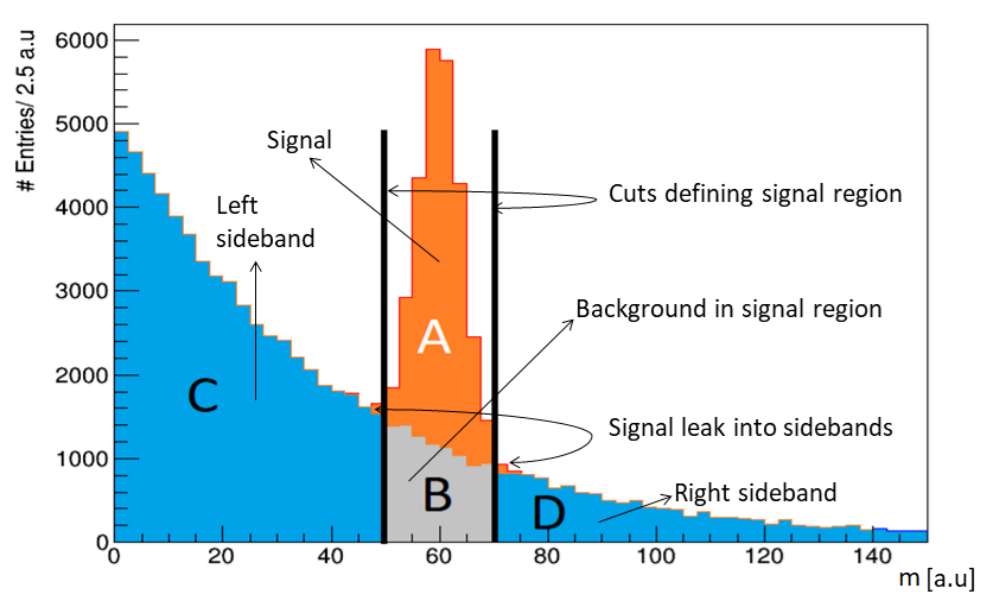
\includegraphics[width=0.7\textwidth]{sideband.png} %插入图片,[]中设置图片大小,{}中是图片文件名
\caption{Sideband} %最终文档中希望显示的图片标题
\label{Sideband} %用于文内引用的标签
\end{figure}

Sideband analysis is a technique used to estimate the background signal in an experiment by studying events in regions of phase space where the signal is expected to be absent or negligible. By comparing the background estimate obtained from these sideband regions with the observed data in the signal region, the contribution of the background to the signal can be estimated and subtracted.
\subsection{Data-Driven method}
数据驱动方法主要借助data来处理本底。这个概念比较宽泛,比如ABCD方法,matrix method等等\newline

Data-driven methods are powerful because they do not rely on simulation, and they can therefore be less susceptible to uncertainties associated with the modeling of the background. However, these methods may be limited by statistical uncertainties in the control sample, and they may require a good understanding of the background processes and the detector response.\newline

Data-driven methods are techniques that use the experimental data itself to estimate the background signal. One example of a data-driven method is the "fake rate" method, which estimates the background signal by measuring the rate at which events with fake particles (i.e., particles misidentified as signal particles) are observed in the data.\newline


\subsubsection{fake rate method}
which estimates the background signal by measuring the rate at which events with fake particles (i.e., particles misidentified as signal particles) are observed in the data.\newline

The fake rate is measured in a control sample that is enriched in events with fake particles, and it is then applied to the signal region to estimate the background. The systematic uncertainty associated with this method is typically estimated by varying the control sample selection criteria and the fake rate measurement.
\subsubsection{control sample method}
which estimates the background signal by studying a sample of events in which the signal is absent or negligible, but the background is expected to be similar to that in the signal region.\newline

Another example of a data-driven method is the "control sample" method, which estimates the background signal by studying a sample of events in which the signal is absent or negligible, but the background is expected to be similar to that in the signal region. The background in the signal region is estimated by scaling the number of events observed in the control sample by the ratio of the expected background in the signal and control samples. The systematic uncertainty associated with this method is typically estimated by varying the control sample selection criteria and the background estimation method.
\subsection{control sample and control region}
\subsubsection{control sample}
It's chosen so as to be rich in background (as predicted by the new physics and SM).The CR does usually not contain only the background we are interested in but also some other contributions.\par
就是我们要研究什么本底过程,就要通过一些条件选择出那个本底过程纯度高的事例样本。

\subsection{control region}
control region, enriched with the dominant background processes.
\subsection{signal region}
The signal region(SR) where the actual measurement of new physics will take place.\par
signal regions, maximising the signal discovery sensitivity.
\subsection{}
\begin{equation}
N_{B G}^{S R}=\left(N_{B G, \text { data }}^{C R}-N_{\cancel{BG}, M C}^{C R}\right) \frac{N_{B G, M C}^{S R}}{N_{B G, M C}^{C R}}
\end{equation}
\section{root}
\subsection{bin}
\subsubsection{underflow and overflow bin}
bin = 0;       underflow bin
bin = 1;       first bin with low-edge xlow INCLUDED
bin = nbins;   last bin with upper-edge xup EXCLUDED
bin = nbins+1; overflow bin
\subsubsection{integral and GetEntries}
integral (include weight),if weight is 1 then integral is equal to GetEntries

\section{琐碎的信息}
The statistical interpretation of the results is based on a simultaneous fit to the
signal and control regions to determine a possible signal contribution and constrain the main backgrounds
with data, taking into account experimental and theoretical systematic uncertainties。\par

The fit is based on a profile-likelihood technique, where systematic uncertainties are allowed
to vary as Gaussian-distributed nuisance parameters (NP) and subsequently acquire their best-fit values.\par


\section{charge asymmetry}
top quarks are produced preferentially in the centre of the LHC’s collisions, while antitop quarks are produced preferentially at larger angles. This is known as a ‘charge asymmetry’\par
Charge asymmetry is similar to a phenomenon measured at the Tevatron collider at Fermilab, known as a ‘forward-backward’ asymmetry. At Tevatron, colliding beams were made of protons and anti-protons, respectively, which led to top and antitop quarks each being produced at non-central angles, but in opposite directions. A forward-backward asymmetry, compatible with improved Standard Model predictions, was observed.

\begin{figure}
    \centering
    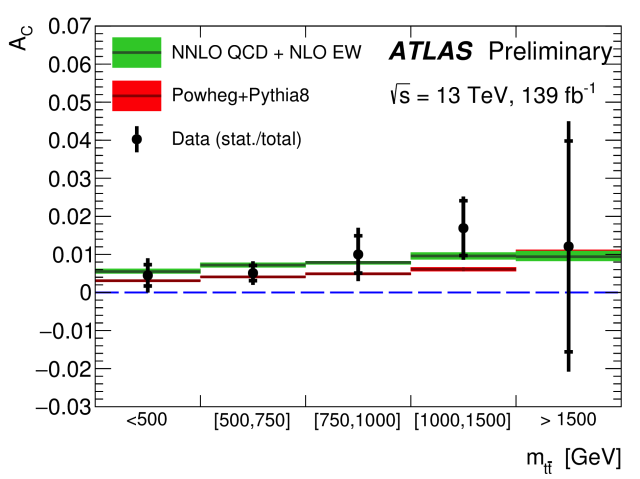
\includegraphics[width=\textwidth,height=10cm]{ATLAS-chargeasymmetry-figure1.png}
    \caption{ATLAS-chargeasymmetry-figure1}
    \label{fig:my_label}
\end{figure}

\section{about observabels}
\subsection{eta,primary\_cluster\_eta,primary\_cluster\_be2\_eta}
\subsubsection{eta}
\subsubsection{primary\_cluster\_eta}
\subsubsection{primary\_cluster\_be2\_eta}
For Electron ID , they almost use primary\_cluster\_be2\_eta (both for selection and for the efficiencies) 
\paragraph{why using primary\_cluster\_be2\_eta}
\begin{itemize}
    \item cluster position is invariant under four-momentum correction ( you don't want  your SFs to depend on verison of the corrections for example )
    \item second layer has highest granularity so its most precise.
    
\end{itemize}



\section{$H\rightarrow Z+\gamma$}      
\url{https://www.quantumdiaries.org/2012/07/03/what-you-need-to-know-about-the-higgs-seminar/}
\subsection{Mass selection}
The search for the Higgs boson depends on its mass. At high mass it can decay to heavy particles with clean signatures, so the high mass region was the first region to see an exclusion. At very high mass the width of the Higgs boson is large, so the events get spread out over a large range, so the searches take a little longer. At low mass the decays get very messy, so we have to pick our decay modes carefully. The cleanest modes are the two photon mode (often called gamma gamma), the ZZ* mode and the WW* mode. Of these three, the gamma gamma and ZZ* modes are the most sensitive, so we can expect to see these presented tomorrow.
\subsection{Reducible and irreducible background}
For each analysis there are two kinds of background, the “reducible” backgrounds where particles fake the particles we are looking for (for example, a high energy electron can look just like a high energy photon) and the “irreducible” backgrounds where particles are the same kind as the ones we are looking for. So when you see plots showing the gamma gamma searches, you can expect to see four categories: gamma gamma (irreducible Standard Model background), jet gamma, jet jet, and “other”. As we make more and more stringent requirements to eliminate these backgrounds we also lose signal events, so we have trade off background rejection against signal acceptance.

\subsection{brazil band plot}  
\url{https://physics.stackexchange.com/questions/13170/particle-physics-plots}\\
\url{https://vixra.wordpress.com/wp-content/uploads/2011/07/hh00-11.jpg}\\
\url{https://indico.in2p3.fr/event/5116/contributions/33052/attachments/26231/32364/2011.07.22_CMS_HiggsComb_EPS_v1.pdf}\\

\url{https://resonaances.blogspot.com/2011/07/higgs-wont-come-out-of-closet.html}\\
\url{https://amva4newphysics.wordpress.com/2016/12/15/brazil-bands-what-are-they/}\\ 
\url{https://arxiv.org/abs/1306.3117}\\  

\subsubsection{explanation}
The experiments produce “Brazil plots”, which show what they expect to see if there is no Higgs, and compare it to what they actually see. The green band shows 1 sigma deviations, the yellow bands show 2 sigma deviations, and then you have to use your imagination to see the remaining bands, and colors. When the green and yellow bands pass below the SM=1 line, and the central black line does too, then the Higgs is excluded in that region to 95% confidence. If the black line stays above the SM=1 line then we haven’t excluded the Higgs boson in that region yet. So when the green and yellow bands fall far below the SM=1 line, but the black line stays above or at the SM=1 line then we accumulate evidence for a Higgs boson.
\end{document}
